%%%%%%%%%%%%%%%%%%%%%%%%%%%%%%%%%%%%%%%%%%%%%%%%%%%%%%%%%%%%%%%%%%%%%%%%%%%%%%%
\chapter{Usage}\label{ChapUsage}
Ash3d 


%%%%%%%%%%%%%%%%%%%%%%%%%%%%%%%%%%%%%%%%%%%%%%%%%%%%%%%%%%%
\section{Preliminary meta-data}\label{ChapUsageSecPrelimData}
Wind files\\
Volcano data\\
Airport/POI data

%%%%%%%%%%%%%%%%%%%%%%%%%%%%%%%%%%%%%%%%%%%%%%%%%%%%%%%%%%%
\section{Running Ash3d on the command-line}\label{ChapUsageSecCommandLine}
The Linux command line provides a more versatile but less
user-friendly environment for running Ash3d simulations.
We do not offer support for installing or running Ash3d
on computers outside the USGS, but we are willing to work
with collaborators who wish to run Ash3d in a more advanced
environment than is possible through the web interface.
Below, we explain how to set up and run a simulation in a
Linux environment. Ash3d is in a state of continuing
development, and we recommend that potential users consult
the authors for updates before following these instructions.

\begin{figure}[htbp]
%\includegraphics[angle=90,scale=0.9]{asharrivaltimesairports_p1.pdf}
\parbox{15cm}{\caption{\label{FigAsh3dOutput}
Examples of model output}}
\end{figure}

\subsection{Model input using an ASCII input file}
The Ash3d executable reads from an ASCII input file that
supplies information on source parameters, output file types,
and other options. A file for a simulation at Redoubt volcano
is illustrated in Appendix \ref{ChapAppendAuxFiles}.
%All elements in blue are
%comments; actual input parameters are shown in black.
If these
files are viewed in a Linux text editor such as \texttt{vi} or
\texttt{gedit}
that converts syntax elements for a shell script into colors,
the same color scheme will be visible, allowing users to easily
discriminate comments from parameters. The input file is further
divided into blocks, delimited with lines of asterisks. Each of
these blocks is described below.

\paragraph{Block 1}: Model grid\\
The lines in this block primarily define the size, shape,
and location of the model domain.
\small
\begin{verbatim}
*******************************************************************************
Spurr                               # Volcano name
1 4 -107.0 50.0 50.0 50.0 6367.47   # Proj flags and params
-154 58                             # x, y of LL corner of grid (km, or deg.)
20.0 6.0                            # grid width and height (km, or deg.)
-152.251 61.299 2.309               # vent location         (km, or deg.)
0.25       0.25                     # DX, DY of grid cells  (km, or deg.)
0.5                                 # DZ of grid cells      (always km)
0.      4.                          # diffusion coefficient (m2/s), Suzuki constant
1                                   # neruptions, number of eruptions or pulses
*******************************************************************************
\end{verbatim}
\normalsize

Line 1 gives either the volcano name or the volcano’s number.
If the number begins with 0 or 1, then the volcano database used is
the Catalog of Active Volcanoes of the World [Siebert et al., 2010].
If the number does not begin with 0 or 1, then the Volcanoes of the
World (VOTW) database is used
[Global Volcanism Program, 2013. Volcanoes of the World, v. 4.9.4 (17 Mar 2021). Venzke, E (ed.). Smithsonian Institution. Downloaded 13 Apr 2021. https://doi.org/10.5479/si.GVP.VOTW4-2013. ].
If the CAVW number is given, Ash3d looks up the eruption source
parameters (ESP) for this volcano in the ESP spreadsheet of
\cite{Mastin09a}. In the example file, the volcano name
is given.

Line 2 gives the projection parameters for this simulation.
Ash3d uses the volcano-ash3d-projection package to specify the
projection and to calculate any needed coordinate transformations.
Documentation for this package can be found at
\url{https://github.com/usgs/volcano-ash3d-projection}
These parameters on Line 2 define the projection for the computational
grid and can be different than the projection used for the numerical
weather prediction (NWP) files. Some of
those NWP models, such as the NOAA National Center for Environmental
Prediction’s (NCEP) Global Forecast System (GFS) model, are run
on a spherical earth, hence the wind vectors are given in a 3-D
grid of latitude, longitude, at pressure levels. Other models, such
as NOAA’s North American Model are run using a grid that is
projected onto a planar coordinate system. After Ash3d reads
the NWP atmospheric data, it must know the type of projection in order
to find the portion of the NWP model grid that lies within the
Ash3d model domain.
Ash3d uses the MetReader library to read the atmospheric data and to
interpolate values from the NWP grid onto the computational grid used
by Ash3d.  MetReader also projects the wind vectors onto the coordinate
system specified in this line.  
The types of NWP model output that
Ash3d can read, and their projection parameters, are given in
Table \ref{tab:ProjOpt}.
The first two parameters on this line are \texttt{latlonflag} and
\texttt{projflag},
where:
\begin{itemize}
 \item \texttt{latlonflag} is an integer whose value is 0 if coordinate system is
projected, 1 if coordinates are in latitude and longitude
 \item \texttt{projflag} is an integer that indicates the projection type
\end{itemize}
Numbers that follow these two integer flags are the projection parameters
that are different for different map projections.
\small
\begin{table}[htbp]
\begin{center}
\begin{tabular}{| c | c | l | l |}
\hline
\texttt{latlonflag} & \texttt{projflag} & Description & Expected parameters\\
\hline
0 & 0 & Non-geographic Cartesian grid & N/A \\
0 & 1 & Polar Stereographic & $\lambda_0$ $\phi_0$ $k_0$ $R_e$ \\
0 & 1 & Albers Equal Area & $\lambda_0$ $\phi_0$ $\phi_1$ $\phi_2$ $R_e$ \\
0 & 1 & UTM & Not yet functional \\
0 & 1 & Lambert Conformal Conic & $\lambda_0$ $\phi_0$ $\phi_1$ $\phi_2$ $R_e$\\
0 & 1 & Mercator & $\lambda_0$ $\phi_0$ $R_e$\\
1 & N/A & Longitude/Latitude & N/A \\
\hline
\end{tabular}
\caption{\label{tab:ProjOpt}Ash3d projection options}
\end{center}
\end{table}
\normalsize
Below are some examples of
this input line. The comment in blue following the hash mark (\#) gives
the projection type.\\
\texttt{0 1 -135.0 90.0 0.933 6371.229 {\color{blue} \#Polar stereographic}}\\
Parameters 3-6 are
$\lambda_0$, the longitude of the projection point;
$\phi_0$, the latitude of the projection point;
$k_0$, the scale factor at the projection point;
and $R_e$, the Earth radius used in kilometers.\\
\texttt{0 4 -95. 25.0 25.0 25.0 6371.229 {\color{blue} \#Lambert Conformal Conic}}\\
Parameters 3-7 are
$\lambda_0$, the longitude of the projection origin;
$\phi_0$, the latitude of the projection origin;
$\phi_1$, the latitude of the first secant;
$\phi_2$, the latitude of the second secant;
and $R_e$, the Earth radius used.

Line 3 gives the x and y (or longitude and latitude if \texttt{latlonflag = 1})
values of the lower
left corner of the grid. These values must be in the same coordinate system
defined by the projection parameters on line 2.

Line 4 gives the model domain width and height, in degrees if latitude and
longitude are used, or kilometers if a projected coordinate system is used.
If latitude and longitude are used and if the width is given as 360 degrees,
then Ash3d uses a periodic grid.

Line 5 gives the vent location, also in the same units as the specified
coordinate system. This line may take either two or three values. The first
two values are required and correspond to the x and y (or longitude and
latitude) coordinates of the vent. A third, optional, value gives to the
volcano’s elevation in
kilometers. If no elevation is given, Ash3d assigns the volcano an elevation
equal to that of the topography at this location, or zero if topography is
not used in this model run. For the web interface, topography is not used.

Line 6 gives the horizontal grid spacing in the model, in kilometers if a
projected grid is used, or degrees if latitude/longitude are used. If the
width and height of the model domain are not an integral number of cell
distances, the location of the upper right corner of the model domain is
adjusted to be an integral number of cell distances from the lower left
corner.

Line 7 specifies the vertical grid structure to be used.  If a number is
given, it is interpreted to be the constant $\Delta z$ for a regular vertical
grid spacing.
The units of this input parameter are always kilometers.
Alternatively, a text string can be given which specifies
different options for a variable spacing of the vertical grid.  This text
string must be one of the following:
\begin{itemize}
\item \texttt{dz\_plin}: for piecewise linear
\item \texttt{dz\_clog}: for constant $\Delta z$ in $\log z$
\item \texttt{dz\_cust}: for custom
\end{itemize}
For each of these variable-$\Delta z$ cases, an additional line must be
provided in the input file immediately after line 7.  For \texttt{dz\_plin},
this line must start with the number of linear segments, followed by the
number of cells and $\Delta z$ in each segments
($n$ $nz_1$ $\Delta z_1$ $nz_2$ $\Delta z_2$ $\cdots$ $nz_n$ $\Delta z_n$).
For \texttt{dz\_clog}, the additional line just contains the number of cells
in $z$.
For \texttt{dz\_cust}, the additional line must start with the vertical
number of cells $nz$, followed by a list of $nz$ values for
$\Delta z$.

Line 8 parameters specify the \textbf{diffusion coefficient $K$} and the \textbf{vertical distribution of mass} in the column, respectively. The diffusion coefficient is specified in $\mathrm{m^2/s}$ and is applied to both the horizontal and vertical diffusivities.  If $K$=0.0,  Ash3d disables the diffusion calculation.  Note that unless Ash3d has been
compiled with the Crank-Nicolson scheme invoked (which requires the lapack library), including diffusion can significantly increase the computation time through the time-step constraints with explicit diffusion solvers.

The vertical distribution of mass may be specified either as a number, or as a text string: \texttt{point}, \texttt{line},
\texttt{profile}, \texttt{umbrella}, and \texttt{umbrella\_air}.  These possibilities are illustrated in Figure \ref{FigVertMassDistFormat}.  If the input is:

\begin{figure}[htbp]\vspace*{-5cm}\hspace*{-2cm}
\includegraphics[angle=0,scale=0.8]{Figures/Scripts/VertMassDist.pdf}
\parbox{15cm}{\caption{\label{FigVertMassDistFormat}
Illustration of vertical mass distributions that can be specified in Ash3d, and the association of these inputs with other aspects of model setup, such as plume height and the configuration of source nodes.
}}
\end{figure}

\begin{itemize}
\item a number: it is assumed to be the Suzuki constant $k$ in Equation \ref{EqSuz}.  Mass distributions for different $k$ are illustrated in Figure \ref{FigVertMassDistFormat}a.
\item \texttt{point}: all mass is placed in a single cell at the plume top (Figure \ref{FigVertMassDistFormat}a).
\item \texttt{line}:  mass is distributed evenly from the vent elevation (if provided) or from sea level (if vent elevation is not provided) to the plume top (Figure \ref{FigVertMassDistFormat}a)
\item \texttt{profile}: each eruptive pulse line in block 2 must be supplemented by an additional line specifying the profile, as described below.
\item \texttt{umbrella} or \texttt{umbrella\_air}: the plume height in Block 2 is interpreted as the height of the umbrella cloud (ash in the overshooting top, above the umbrella cloud, is assumed to collapse gravitationally back into the umbrella rather than being advected horizontally by winds at that altitude).  This source type is most appropriate for eruptions of VEI=6 and larger, and may bed appropriate for some VEI 4 or 5 eruptions \cite{Mastin20}.  Source nodes for these cases consist of a column of nodes extending from the vent elevation (if provided) to 75\% of the umbrella top height, or from sea level (if vent elevation is not provided) to 75\% of the umbrella top height. From 75\% to 100\% of the umbrella top height, source nodes consist of a matrix 3x3 in plan view (Figure \ref{FigVertMassDistFormat}b).  Within the height range of the 3x3 matrix, from the vent outward to the edge of the expanding umbrella cloud, radial wind vectors are added to the ambient wind field.  The magnitude of the radial wind vectors is calculated using corrected Equations (2) and (3) of \cite{Costa13}, and is proportional to the mass eruption rate.
The only difference between ``umbrella'' and ``umbrella\_air'' is that the latter is used only for simulations of airborne ash, where a single grain size is used, and the volume of ash is assume to equal  5\% of the total erupted volume.  Only one eruptive pulse may be specified when the umbrella source is used.
\item neither a number nor one of the above types: Ash3d assumes this source type is a user-specified custom source type.  These are described in detail in section \ref{SecOptionalModulesUserCust}
\end{itemize}

Line 9 gives the number of eruptions or eruptive pulses in the simulation. The eruptions or eruptive pulses may be either contiguous or non-contiguous in time. Their duration should not be shorter than the average time step in the model (about a minute).

\paragraph{Block 2}: Eruptive pulses\\
For source types suzuki, point, line, umbrella, or umbrella\_air,
the number of lines in this block equals the number of eruptions or eruptive pulses specified in line 9 of Block 1. A line of input for these types contains three integers followed by four real numbers, for example:
\small
\begin{verbatim}
*******************************************************************************
1992 08 19   1.0   3.5     13.7   0.014
*******************************************************************************
\end{verbatim}
\normalsize

The first four numbers represent the year, month, day and hour (UTC) of the start of the eruption. The following three numbers represent the eruption duration in hours, the plume height in kilometers above sea level, and the erupted volume in cubic kilometers dense-rock equivalent (DRE). Ash3d converts the erupted volume to a mass assuming a magma density of 2500 $\mathrm{kg/m^3}$. If the year is zero as in the example input file, the model is run in forecast mode where the hour is interpreted as the number of hours after the start time of the wind files. In addition, if the duration, plume height, or erupted volume is negative, it is replaced with the default ESP value for that volcano from the spreadsheet of \cite{Mastin09b}.

If the source type is ``profile'', then the eruption lines are read as three integers, four real numbers, and an integer where instead of the erupted volume, the last two numbers are the $\Delta z$ and number of $z$-points defining the profile.  This type of source type must have a line following with the list of eruptive volume values for each of the $\Delta z$ segments.  An example of this type is given below.
\small
\begin{verbatim}
*******************************************************************************
1992 08 19   1.0   3.5     13.7   0.5 14
0.0 0.0025 0.0025 0.005 0.01 0.015 0.02 0.025 0.025 0.01 0.01 0.005 0.005 0.005
*******************************************************************************
\end{verbatim}
\normalsize

\begin{figure}[htbp]
%\includegraphics[angle=90,scale=0.9]{asharrivaltimesairports_p1.pdf}
\parbox{15cm}{\caption{\label{FigSourceOptions}
Example of source term options}}
\end{figure}
If the source type is not recognized, Ash3d just reads the first line of this
block which must have at a minimum three integers for the year, month and day,
followed by three real values for the hour, duration and height.  There may
be more values on the eruption source line and potentially additional lines to
read for the custom sources, but this is parsed later after the remaining blocks
are read.

\paragraph{Block 3}: Wind files and simulation time\\
Line 1 of block 3 gives at least two integers, \texttt{iwind} and \texttt{iwindFormat}.
The first number (\texttt{iwind}) specifies the structure of the windfiles and can
have the following values:
1=1-D wind sounding(s),
2=3-D gridded ASCII files,
3=a single NWP file (all variable data for all steps in one file),
4=multiple NWP files (all variable data for one step in individual files),
5=non-standard files that require hard-wired paths.
%\begin{center}
%\begin{tabular}{| c | l |}
%\hline
%\texttt{iwind} & Description \\
%\hline
%1& 1-D wind sounding(s) \\
%2& 3-D gridded ASCII files \\
%3& a single NWP file (all variable data for all steps in one file) \\
%4& multiple NWP files (all variable data for one step in individual files)\\
%5& non-standard files that require hard-wired paths \\
%\hline
%\end{tabular}
%\end{center}

The distinction between \texttt{iwind}=3 and \texttt{iwind}=4 has been
relaxed and these are now interchangable.
Ash3d attempts to read two more integer values on line 1
of this block: a grid ID, and a format code.  The grid code is the NCEP grid
ID described at \url{http://www.nco.ncep.noaa.gov/pmb/docs/on388/tableb.html}
and the format code must be either 1 (ASCII), 2 (NetCDF), or 3 (GRIB v1 or v2).
If these values are not provided, the grid code is assigned if known from the
NWP product given by \texttt{iwindFormat} and the data format code is assumed to
be 2=NetCDF.  The combinations of \texttt{iwind} and \texttt{iwindFormat} are shown in
Table \ref{tab:MetOptions}.

\small
\begin{table}[htbp]
\begin{center}
\begin{tabular}{| c | c| c | c | l |}
\hline
\texttt{iwind} & \texttt{iwindFormat} & \texttt{grid} & \texttt{data} &Description \\
\hline
1& & & & 1-D wind sounding(s) \\
\hline
 &1&n&1& User-specified \\
 &2&n&1& global radiosonde data \\
\hline
2& & & &3-D gridded ASCII files \\
 & & & &Not implemented\\
\hline
3& & & &one NWP file for all data\\
4& & & &one NWP file per time step\\
\hline
 & 0& &2&User-defined via template\\
 & 3&221&2/3&North American Regional Reanalysis NARR\\
 & 4&221&2/3&NAM Regional North America\\
 & 5&216&2/3&NAM Regional Alaska\\
 & 6&104&2/3&NAM N. Hemisphere\\
 & 7&212&2/3&NAM Regional CONUS\\
 & 8&218&2/3&NAM Regional CONUS\\
 & 9&227&2/3&NAM Regional CONUS\\
 &10&242&2/3&NAM Regional Alaska\\
 &11&196&2/3&NAM Regional Hawaii\\
 &12&198&2/3&NAM Regional Alaska\\
 &13& 91&2/3&NAM Regional Alaska\\
 &14&   &2/3&NAM Regional CONUS \\
 &20&  4&2/3&GFS\\
 &21&  3&2/3&GFS\\
 &22&193&2/3&GFS\\
 &23&  2&2/3&NCEP-DOE Reanalysis 2\\
 &24&   &2/3&NASA-MERRA-2 Reanalysis\\
 &25&  2&2/3&NCEP/NCAR Reanalysis 1\\
 &28&170&2/3&ECMWF ERA-Interim Reanalysis\\
 &32&   &2/3&Air Force Weather Agency subcenter = 0\\
 &33&   &2/3&CCSM3.0 Community Atmosphere Model\\
 &40&   &2/3&NASA GEOS-5 Cp\\
 &41&   &2/3&NASA GEOS-5 Np\\
 &50&   &2/3&WRF - output\\
\hline
5& & & &files that require hard-wired paths \\
\hline
 &25&  2&2/3&NCEP/NCAR Reanalysis 1\\
 &26& 45&2/3&JRA-55\\
 &27&  2&2/3&NOAA-CIRES 20th Century Reanalysis\\
 &29&   &2/3&ECMWF ERA5 Reanalysis\\
 &30&   &2/3&ECMWF ERA-20C Reanalysis\\
\hline
\end{tabular}
\caption{\label{tab:MetOptions}Ash3d options for wind data}
\end{center}
\end{table}
\normalsize

If \texttt{iwind}=1, Ash3d reads from one or more ASCII files of a 1-D wind sounding.
%format shown in Table \ref{}.
This option can be used if no numerical weather prediction
data are available or if data from a single radiosonde measurement is deemed more
reliable than NWP model results.
If \texttt{iwindFormat}=1, then Ash3d expects the user-provided files to have a format
of 3 header lines, followed by three or more columns of data.  The format specification
is documents in the MetReader User's Guide, but also outlined in the
Appendix \ref{ChapAppendAtmosDataFormat1d}.

If \texttt{iwindFormat}=2, then Ash3d expects the 1-D profile to be from the global
radiosonde data available from \url{https://ruc.noaa.gov/raobs/} or from
\url{http://weather.uwyo.edu}.  Details on the particular formats Ash3d is able to
read is described in Appendix \ref{ChapAppendAtmosDataFormat1d}.

Since there is no grid for these data, \texttt{igrid}, if provided, is interpreted to
be the number of stations with 1-D data.  This is currently not yet implemented.

When \texttt{iwind}=2, Ash3d reads a 3-D atmospheric fields in ASCII format that is converted from
NetCDF format using a Java script that was originally written before Ash3d was
modified to read NetCDF files directly. This option is no longer used.
\texttt{iwind}= 3 or 4 indicates that the atmospheric files contain 3-D time-series
data.  Orginally, \texttt{iwind}=3 was used for indicating that all data were stored in
a single file with multiple time steps, and \texttt{iwind}=4 was for multiple NetCDF files,
each for one time step.  This distinction is deprecated as currently, all data
files provided with \texttt{iwind}= 3 or 4 are evaluated for the time steps available.
This then can accommodate the occasional NWP products that provide data in a
multiple-file, multiple-time-step format.

%The two options were
%created to accommodate different posting conventions for different kinds of wind
%files. For example, Global Forecast System output files posted at Unidata
%(\url{http://unidata.ucar.edu}) for current and forecast conditions include a separate
%file for every three-hour time step. Alaska 11km North American Model forecasts
%posted at Unidata are given as a single file for multiple time steps.
%The second parameter, \texttt{iwindFormat}, indicates the type of NWP file to be read. The
%values of \texttt{iwindFormat} for each NWP file type are listed in Table \ref{}.
Line 2 gives the integer \texttt{iHeightHandler}, which indicates how Ash3d should respond
if it finds that the plume height exceeds the highest level in the NWP model.
Numerical weather prediction models give 3-D atmospheric fields with the vertical coordinate
in pressure levels. For the GFS 0.5 degree model, the highest pressure level is ~40 kPa,
which corresponds to about 50 km altitude. The atmospheric conditions at higher altitude is
unknown from these models. If the input plume height is higher than the highest
altitude in the NWP model, Ash3d responds in one of the following ways: if
\texttt{iHeightHandler}=1, Ash3d execution stops and writes an error message to standard output
and the log file.
If \texttt{iHeightHandler}=2, Ash3d continues execution and uses the wind vectors in the
top-most pressure level in all higher pressure levels. Temperature is calculated for these
higher altitudes using the US Standard Atmosphere. Ash3d also writes a warning
message to standard output and to the log file,

Line 3 gives the simulation time in hours. The simulation time is assumed to start
at the time of the first eruption or eruptive pulse. Ash3d checks the time duration
of the atmospheric files to ensure that the entire simulation time is contained within
the scope of provided files.

Line 4 is a ``yes'' or ``no'' parameter that specifies whether to stop computation
when 99\% of the the erupted mass has deposited. Setting this parameter to ``yes''
allows for faster execution if users are primarily interested in simulating
deposition. If simulating ash-cloud transport is of primary interest, users may
prefer to set this parameter to ``no''.

Line 5 specifies \texttt{nwindfiles}, the number of atmospheric files to be read.
%If more than one file is to be read, the parameter iwind in Block 3, line 1, must equal 4.
%Ash3d assumes in that case that each wind file contains a single time slice.
Ash3d examines the time stamp of all the steps of all the atmospheric files to ensure
that the start time and end time of the simulation are within the scope of the
provided files.

\paragraph{Block 4}: Output options\\
Most lines in this block specify types of output options that can be written at
specific output steps.
Lines 1-15 require ``yes'' or ``no'' to indicate whether a particular type of output
should be written. These types of output are listed in Table \ref{tab:OutputOptions}
along with the names of files written out.
\small
\begin{table}[htbp]
\begin{center}
\begin{tabular}{|r|l|l|l|l|}
\hline
Line & Output type&Variable&units & File names\\
\hline
 1&ESRI\textsuperscript{\tiny\textregistered} ASCII &final deposit thickness&$\mathrm{mm}$&DepositFile\_\_\_\_\_final.dat\\
 2&KML&final deposit thickness&$\mathrm{mm}$&deposit\_thickness\_mm.kml\\
  & & &$\mathrm{inches}$&deposit\_thickness\_inches.kml\\
 3&ESRI\textsuperscript{\tiny\textregistered} ASCII &deposit at specified times&$\mathrm{mm}$&Deposit\_xxx.xxhrs.dat\\
 4&KML&deposit at specified times&$\mathrm{mm}$&deposit\_thickness\_mm.kml\\
  & & &$\mathrm{inches}$&deposit\_thickness\_inches.kml\\
 5&ESRI\textsuperscript{\tiny\textregistered} ASCII &ash-cloud concentration&$\mathrm{mg/m^3}$&CloudConcentration\_xxx.xxhrs.dat\\
 6&KML& ash-cloud concentration&$\mathrm{mg/m^3}$&CloudConcentration.kml\\
 7&ESRI\textsuperscript{\tiny\textregistered} ASCII&ash-cloud height&$\mathrm{km}$&CloudHeight\_xxx.xxhrs.dat\\
 8&KML&ash-cloud height&$\mathrm{km}$&CloudHeight.kml\\
 9&ESRI\textsuperscript{\tiny\textregistered} ASCII&ash-cloud load at specified times&$\mathrm{T/km^2}$&CloudLoad\_xxx.xxhrs.dat\\
10&KML&ash-cloud load at specified times&$\mathrm{T/km^2}$&CloudLoad.kml\\
11&ESRI\textsuperscript{\tiny\textregistered} ASCII&deposit arrival times&$\mathrm{hours}$&DepositArrivalTime.dat\\
12&KML&deposit arrival times&$\mathrm{hours}$&ashfall\_arrivaltimes\_hours.kml\\
13&ESRI\textsuperscript{\tiny\textregistered} ASCII&cloud arrival times&$\mathrm{hours}$&CloudArrivalTime.dat\\
14&KML&cloud arrival times&$\mathrm{hours}$&cloud\_arrivaltimes\_hours.kml\\
15&&consolodated output file&&specified as input\\
\hline
\end{tabular}
\caption{\label{tab:OutputOptions}Block 4 options for output data}
\end{center}
\end{table}
\normalsize
The ESRI\textsuperscript{\tiny\textregistered} ASCII files noted in Table \ref{tab:OutputOptions}.
are ASCII files written in a format that
can be directly imported into Arc\textsuperscript{\tiny\textregistered}
GIS products for display.
These files can also be easily converted to a format suitable for plotting with
Generic Mapping Tools (GMT) with the command:
\begin{verbatim}
gmt grdconvert DepositFile___final.dat=ef out.grd
\end{verbatim}
These files contain a six-line
header followed by a 2-D matrix containing values of, for example deposit thickness.
The header looks like:
\small
\begin{verbatim}
NCOLS 140
NROWS 140
XLLCORNER -2616390.
YLLCORNER 1742330.
CELLSIZE 5000.000
NODATA\_VALUE -9999.
\end{verbatim}
\normalsize

The parameters \texttt{XLLCORNER} and \texttt{YLLCORNER} give the coordinates
of the lower-left
corner of the model domain in meters (if it is a projected grid) or degrees (if
the grid is latitude/longitude). The cell size is in the same units as the corner
coordinates. Note: the cell size printed out in these headers is the spacing in
x only. Ash3d can generate grids whose x and y spacing are unequal, and this is
typically the case for simulations generated using the web interface. But Arc
products require the x and y spacing to be equal. Note: If you plan to import
the ESRI\textsuperscript{\tiny\textregistered} ASCII files into
Arc products, make sure to specify equal x and y cellsize
on line 6 of block 1.
The kml files are written using Keyhole Markup Language and can be opened by
Google Earth\textsuperscript{\tiny\textregistered} or other virtual globe
software. The kml files can be zipped using the
following Linux command, which reduces file size by about 90-95\% and creates a
kmz file that can also be opened in Google Earth:
\texttt{zip –r CloudLoad.kmz CloudLoad.kml}

The consolodated output file option specified in line 15 of Table \ref{tab:OutputOptions}
serves several purposes.  It is designed to store the store the full ash concentration
for each grainsize bin
of all cells at specified time steps in a format specified in line 16.  Current options
for this output format is ``ascii'', ``binary'', or ``netcdf''.  If ``netcdf''
is specified, this output file can serve as a restart file, allowing a failed or
suspended job to continue from the last output step.  The NetCDF file contains
the full contents of the input file used to run the job to facilitate its
role as a restart file.  
The NetCDF file also contains the various output variables that can be selected
in lines 1-14 above.  These include the following 2-D variables;
depothick, depotime, ash\_arrival\_time, ashcon\_max, cloud\_height,
cloud\_load, radar\_reflectivity, cloud\_bottom, as well as two variables
which are a function of grainsize; depocon and ashcon.
Optionally, an additional integer specifier can be included on
line 15 to indicate if this consolodated output file should only contain the
2-D variables, which dramatically reduces the size of the output file, at the
expense of losing restart capibilities.
If this specifier is either absent or is 1, then the 3-D concentrations are written.
If it is 2, then only the 2-D output products are written.

Specifying ``netcdf'' in line 16 provides the most general output product for post
processing.  If line 16 contains ``asciii'', then data are written in ASCII format
to files names ``3d\_tephra\_fall\_xxx.dat'' where ``xxx'' is the output hour marker.
The output data are in column format in the following order: x (or lon), y (or lat), z,
total concentration (in $\mathrm{kg/km^3}$).
If ``binary'' is specified, then then total ash concentration is written to the files
``3d\_tephra\_fall\_xxx.raw'' where ``xxx'' is the output hour marker.
Similarly, the deposit thickness is written to the files ``2d\_tephra\_depo\_xxx.raw''.
The following
code sections shows how the data are written:
\begin{verbatim}
open(unit=20,file='3d_tephra_fall_'//cio//'.raw', &
     status='replace', &
     access='direct',recl=4*nxmax*nymax*nzmax)
write(20,rec=1)(((ashcon(i,j,k),i=1,nxmax),j=1,nymax),k=1,nzmax)
close(20)
open(unit=21,file='2d_tephra_depo_'//cio//'.raw', &
     status='replace', &
     access='direct',recl=4*nxmax*nymax)
write(21,rec=1)((DepositThickness(i,j),i=1,nxmax),j=1,nymax)
close(21)
\end{verbatim}
To read these files, you will need to know the values for \texttt{nxmax},
\texttt{nymax}, and \texttt{nzmax}.  Although the default precision for
calculations in Ash3d is \texttt{real*8}, the default output precision is
\texttt{real*4} in order to reduce output file size.  This can be changed, if desired
by editing the code in module \texttt{precis\_param} to set the internal
precision (\texttt{ip}) and the output precision (\texttt{op}).
See \ref{ChapSoftwareStructure}
for more details on editing these and other compile-time parameters.

The 3-D ash concentration file specified in line 15 of Table \ref{tab:OutputOptions}
contains the full
3-D distribution of each grain size in the model domain at specified times.
The following lines complete this block of input:

Line 17 gives nWriteTimes, the number of times data are to be written out to the
files above. Data may be written out at uneven intervals (e.g. 0.2, 3, 3.4, and
12 hours after the eruption start) or at even intervals (e.g. every two hours,
starting 2 hours after the eruption start).

Line 18 gives the times at which output is written:
If \texttt{nWriteTimes}$>0$, line 18 should contain nWriteTimes numbers, in increasing order,
which specify the times in hours after the start of the eruption at which the above
data are to be written.
If \texttt{nWriteTimes}$=-1$, line 18 should contain a single number indicating the time
interval in hours between write times.

\paragraph{Block 5}: Input wind files
This block should contain a number of lines equal to \texttt{nWindFiles} (Block 3, line 5).
For the case of \texttt{iwind}$=5$, \texttt{nWindFiles} shoud be 1 and Block 5 line 1
should be the path to the top-level directory of that product.  For example, for the
NCEP $2.5^{\circ}$ Reanalysis files stored as
\begin{verbatim}
/data/WindFiles/NCEP
|-- 2016
|   |-- air.2016.nc
|   |-- hgt.2016.nc
|   |-- omega.2016.nc
|   |-- uwnd.2016.nc
|   `-- vwnd.2016.nc
|-- 2017
    |-- air.2017.nc
    |-- hgt.2017.nc
    |-- omega.2017.nc
    |-- uwnd.2017.nc
    `-- vwnd.2017.nc
\end{verbatim}
only \texttt{/data/WindFiles/NCEP} should be given on line 1.
Unless \texttt{iwindFormat} (Block 3, line 1) is 1 or 2, these files should be in
either NetCDF or GRIB
format and should consist of output from one of the model types listed in
Table \ref{tab:MetOptions}.
Each line gives the file name and path. In the example file, Ash3d reads a single
wind file named latest.nc, located in the subdirectory Wind\_nc. Ash3d opens this
file and does a preliminary read to ensure that it covers the time period and
geographic region specified in input.

\paragraph{Block 6}: Arrival times at airports
The input lines in this block specify whether arrival times and other information
at specific locations are to be written to output. Normally, Ash3d reads from a
text input file containing the latitude and longitude (or x and y locations) of
a list of points. For the web interface, this is a global list of airports, but
when hand-editing the ASCII input file, other lists, such as sample locations, may
also be specified. Ash3d can then generate either text or kml files listing the
subset of these locations where ash was deposited or where the cloud passed overhead.
Ash3d can also write out the grain-size distribution of points at those locations.
All but line 4 require ``yes'' or ``no'' parameters.

Line 1 indicates whether to write out ash arrival times at these locations to an
ASCII file. If ``yes'' is given, an output file is generated called
\texttt{ash\_arrivaltimes\_airports.txt}
in the format shown in Figure \ref{FigAshArrivTimeFormat}.

\begin{figure}[htbp]\vspace*{-5cm}\hspace*{-2cm}
\includegraphics[angle=90,scale=0.9]{Figures/Chap_Usage_asharrivaltimesairports_p1.pdf}
\parbox{15cm}{\caption{\label{FigAshArrivTimeFormat}
Example of output file \texttt{ash\_arrivaltimes\_airports.txt}
}}
\end{figure}

Line 2 indicates whether the ASCII output file should give a grain-size distribution
of the tephra deposit at each location.

Line 3 indicates whether to write out a kml file showing the locations that will be
impacted by ash. If ``yes'' is given, a file named
\texttt{ash\_arrivaltimes\_airports.kml} is generated
that plots each impacted location as a red placemarks as shown in
Figure \ref{FigAsh3dOutput}.
Additionally, files for each impacted airport are generated that contain the data
for the ash accumulation as a function of time.  These files are named
\texttt{depTS\_xxxx.dat} (where \texttt{xxxx} is the airport number in order of
time of ash arrival) and have two columns containing hour and ashfall thickness
in $\mathrm{mm}$.  Additionally, a gnuplot script is written for each of these
airport locations so that time-series plots of ashfall accumulation can be imbedded
in the kml files in post-proceesion.

Line 4 gives the name and path of the file containing airports or other locations
of interest.  The format of this file must contain four columns with the location
information (latitude, longitude, x, y), followed by the 3-character IATA airport
code, then a 42-character descriptive string such as location.  While the IATA
code is currently not used in any output products, the descriptive
string is use in ash arrival output products.  An example of the expected format
for the airport file is given below.
\small
\begin{verbatim}
#   Latitude   Longitude           x           y  Code Location
    41.60833   -88.09417     0.00000     0.00000  II2  Lewis University Airport, IL
    34.68861   -85.29056     0.00000     0.00000  GA1  Barwick Lafayette Airport, GA
    58.36528  -152.69667     0.00000     0.00000  A33  Hidden Lake, AK
\end{verbatim}
\normalsize
In this case, airports with latitude and longitudes are given, but the x and y
columns are filled with 0.0 as a place-holder.  If the computational grid is
Lon/Lat, then these airport coordinates will be used.  If the computational 
grid is projected, then the x and y columns can be filled with the appropriate
values for the coordinate system used.  Alternatively, the internal projection routines
can be used to generate the x and y values from the latitude and longitude columns.
This would over-write any values read in from the x and y columns of the file.
To have specify that Ash3d should calculate the projected coordinates, line 5 of
this block can be set to ``yes''.  Ash3d would then convert the latitude and longitude
to the projected system specified in Block 1, line 2.  If this line is ``no'' and 
if the computational grid is projected, then the x and y columns of the airport
file are used and the latitude and longitude columns are ignored.  

Included with Ash3d is an internal list of 6117 global airports with IATA codes,
locations, and coordinates.  By default, this is a filled variable at compile-time,
but optionally can be read at run-time from the
file \texttt{/opt/USGS/Ash3d/share/GlobalAirports\_ewert.txt}.  If Line 4 of this
block is empty, or has the word ``internal'', then this built in list of global
airports is used.  If an airport file name is provided, then this internal list
is replaced.  Alternatively, if the first character of the file name provided is
`+', then the contents of the file are appended to the internal global list.  For
example, if the block had the following form:
\small
\begin{verbatim}
****************** BLOCK 6 ***************************************************
yes              # Write out ash arrival times at airports to ASCII FILE?
no               # Write out grain-size distribution to ASCII airport file?
yes              # Write out ash arrival times to kml file?
+PointOfInt.txt  # Name of file containing aiport/POI locations
yes              # Have libprojection calculate projected coordinates?
*******************************************************************************
\end{verbatim}
\normalsize
then the global airport list would be extended by the contents of PointOfInterest.txt
with the x and y columns ingnored in favor of the longitude and latitude or
internally projected mappings.  The maximum number of airports is currently set
to 10,000.

\paragraph{Block 7}: Grain size groups
Ash3d can run an unlimited number of grain sizes, although the required run time
increases roughly in proportion to the number of grain sizes. To reduce model run
time, Ash3d stops calculations for individual grain sizes once they have left the
simulation domain, either advected out the sides or deposited.  A grain size bin is
flagged as having left the simulation domain when $1 \mathrm{g}$ or less remains of
that grain size bin throughout the model domain.
When simulating ash clouds, one very small grain size ($0.01 \mathrm{mm}$ for
example) with a
very low settling velocity is frequently adequate to display general cloud movement.
When simulating deposits, it is best to use at least a half dozen grain sizes: fewer
grain sizes tend to produce secondary thickness maxima as an artifact
\cite{Mastin12}.

Line 1 of Block 7 consists first of an integer giving the number of size bins
(\texttt{nsize}).
Optionally, a second integer can be provided which specifies the fall model to be used
(FV\_ID).
\begin{table}[htbp]
\begin{center}
\begin{tabular}{| c | l | c | }
\hline
\texttt{FV\_ID} & Fall model & Expected parameters\\
\hline
N/A & Wilson/Huang & $F \,[0.44]$ \\
0 &  Tracer only & N/A \\
1 &  Wilson/Huang & $F\, [0.44]$ \\
2 &  Wilson/Huang with slip-flow & $F\, [0.44]$ \\
3 &  Pfiffer mod. of Wilson/Huang & $F\, [0.44]$ \\
4 &  Ganser & $F,G \,[0.44,1.0]$ \\
5 &  Stokes flow with slip-flow & N/A \\
\hline
\end{tabular}
\caption{\label{tab:FallModelOpt}Particle fall models}
\end{center}
\end{table}

If FV\_ID is not given or FV\_ID=1, the Wilson and Huang \cite{Wilson79}
model is used.
If FV\_ID=2, the Wilson and Huang model with a slip-flow correction is used \cite{Seinfeld06}.
If FV\_ID=3, the modification to the Wilson and Huang model outlined
by \cite{Pfeiffer05} is used. If FV\_ID=4, the model of \cite{Ganser93} is used. If
FV\_ID=5, Stokes flow for spherical particles with a slip-flow correction is used.
Optionally, fall velocities can be deactivated by setting FV\_ID=0.  In \ref{tab:FallModelOpt},
the default values for $F$ and $G$ are shown in bracket which Ash3d uses if the corresponding
columns of Block 7 are absent.

The first line of this block is followed by \texttt{nsize} lines, one for each bin size.
These lines may contains two, three, four or five numerical parameters:

If two parameters: Ash3d reads the first as the mass fraction of that size bin, and
the second as the settling velocity in $\mathrm{m/s}$. Ash3d uses this as a constant settling
velocity, independent of elevation or fall velocity model. For example, the following block
specifies two grain classes, 70\% with a fall velocity of 0.01 $\mathrm{m/s}$ and 
30\% with a fall velocity of 1.0 $\mathrm{m/s}$.
\small
\begin{verbatim}
*******************************************************************************
2                            # Minimalist Grain-size specification
1.00 0.3
0.01 0.7
*******************************************************************************
\end{verbatim}
\normalsize
If three parameters: Ash3d reads the first as grain size in millimeters, the second
as the mass fraction, and the third as the density in $\mathrm{kg/m^3}$.
Ash3d calculates settling
velocity of these particles assuming a shape factor ($F$) of $0.44$, which is the average
of values measured by Wilson and Huang \cite{Wilson79}. The settling velocity in this case
depends on air density and viscosity. Air density is calculated from the pressure
and temperature at a
given elevation (obtained from the NWP model data). The viscosity is calculated from
Sutherland’s Law \cite{Jacobson05}, p. 201.  The example below shows the grain-size
distribution used for the airborne runs on the Ash3d webserver.
\small
\begin{verbatim}
*******************************************************************************
1                            # Web server airborne case
0.0100 1.00 2000.
*******************************************************************************
\end{verbatim}
\normalsize
If four parameters: Ash3d reads the first three as before, and the last as a
shape factor.  For the Wilson and Huang class of models (FV\_ID=1,2, or 3)
the shape factor, $F$, is defined as $F=(b+c)/2a$, where $a$, $b$, and $c$ are the
semimajor, intermediate, and semiminor diameters of an ellipsoid.
\small
\begin{verbatim}
*******************************************************************************
14 2                         # McGimsey Spurr
4       0.07303974221267455 800.0  0.8
2       0.07303974221267455 800.0  0.8
1       0.05907626208378088 800.0  0.8
0.5     0.04403866809881848 800.0  0.8
0.25    0.06337271750805586 1083.0 0.8
0.125   0.25026852846401720 1790.6 0.8
0.0625  0.12567132116004298 2000.0 0.8
0.03125 0.11815252416756176 2000.0 0.8
0.01563 0.08700322234156821 2000.0 0.8
0.00781 0.05692803437164339 2000.0 0.8
0.0039  0.03114930182599356 2000.0 0.8
0.00195 0.01396348012889366 2000.0 0.8
0.00098 0.00322234156820623 2000.0 0.8
0.00049 0.00107411385606874 2000.0 0.8
*******************************************************************************
\end{verbatim}
\normalsize
For the Ganser model, shape is characterized by the sphericity, $\phi$, defined as the
ratio of the surface area of a sphere with equivalent volume to the actual surface area
of the particle.  If four parameters are provided with the Ganser model specified, then
Ash3d interprets the fourth term as the Wilson and Huang shape paramter $F$, but
additionally assumes $b=c<a$ (i.e. only prolate elipsoids) so as to calculate area and
volume of the particles and thereby $\phi$.
If a fifth parameter is given, then it is interpreted to 
be the ratio $c/b$, which allows oblate elipsoids to be specified.
\small
\begin{verbatim}
*******************************************************************************
4 4                         # Ganser
0.125   0.2 1790.6 0.8 1.0
0.0625  0.2 2000.0 0.8 1.0
0.03125 0.3 2000.0 0.3 1.0  # needles
0.03125 0.3 2000.0 0.9 0.2  # flakes
*******************************************************************************
\end{verbatim}
\normalsize
See \ref{ChapAppendFallDynamics} for further discussion on the implementation and subtelties of the various
fall models.

The grain-size specifications can be used to describe multiple populations of particles
if desired.  For example, the default grain-size distribution used on the Ash3d
web-server for deposit simulations contains 6 bins
($1 \mathrm{mm} \Rightarrow 88 \mathrm{\mu m}$) describing the primary grain-size distribution
but also includes 4 bins to describe a distribution of aggregates with a lower density
and more equant shape.
\small
\begin{verbatim}
*******************************************************************************
12                           # Web-server dep
2        0.06118        800     0.44
1        0.07098 1040    0.44
0.5      0.22701 1280    0.44
0.25     0.21868 1520    0.44
0.1768   0.05362 1640    0.44
0.125    0.04039 1760    0.44
0.088    0.02814 1880    0.44
0.2176   0.018   600     1.0
0.2031   0.072   600     1.0
0.1895   0.12    600     1.0
0.1768   0.072   600     1.0
0.1649   0.018   600     1.0
*******************************************************************************
\end{verbatim}
\normalsize

If the diameter of the last grain-size bin is negative, then the last grain-size line
is reinterpreted to allow a log-normal grain-size distribution.
In this case, the commonly-used logrithmic specification of grain-size,
$\phi=-\log_2 d$ (with $d$ in $\mathrm{mm}$), is used where $\phi$ is normally
distributed.
The second and third values of this last line
are interpreted to be the mean ($\mu_{\phi}$)
and standard deviation ($\sigma_{\phi}$).
The remaining mass fraction not accounted for in the previously specified
bins is distributed among all the bin according to 
\begin{equation}
N=\frac{1}{\sigma_{\phi} \sqrt{2 \pi}}
\exp{\left[-\frac{1}{2} \left(  \frac{\phi-\mu_{\phi}}{\sigma_{\phi}}  \right)^2 \right]}
\end{equation}
Note that using the log-normal distribution assumes that all the grain-size bins
are part of the primary grain-size distribution with no bins representing special
classes such as aggregates.  Secondly, Ash3d assumes that the bins are listed in
order from smallest to largest and will sort all grain sizes to ensure this order.
This sorting would interfere with multiple grain populations if an aggregate
population or a flake/needle distinction is specified.  The example below shows
a log-normal grainsize distribution with a mean of $\mu_{\phi}=5.5$ and a standard
deviation of $\sigma_{\phi}=2$.  Note that this grainsize order will be reversed.
\small
\begin{verbatim}
*******************************************************************************
15 2                         # Gaussian
4       0.000 800.0  0.8
2       0.025 800.0  0.8
1       0.100 800.0  0.8
0.5     0.025 800.0  0.8
0.25    0.0 1083.0 0.8
0.125   0.0 1790.6 0.8
0.0625  0.0 2000.0 0.8
0.03125 0.0 2000.0 0.8
0.01563 0.0 2000.0 0.8
0.00781 0.0 2000.0 0.8
0.0039  0.0 2000.0 0.8
0.00195 0.0 2000.0 0.8
0.00098 0.0 2000.0 0.8
0.00049 0.0 2000.0 0.8
-1 5.5 2
*******************************************************************************
\end{verbatim}
\normalsize

Several of the above example grain-size distributions are shown in 
Figure \ref{FigInputGSD} 
illustrating how this feature can be used to implement bimodal distributions.
\begin{figure}[htbp]
\begin{center}
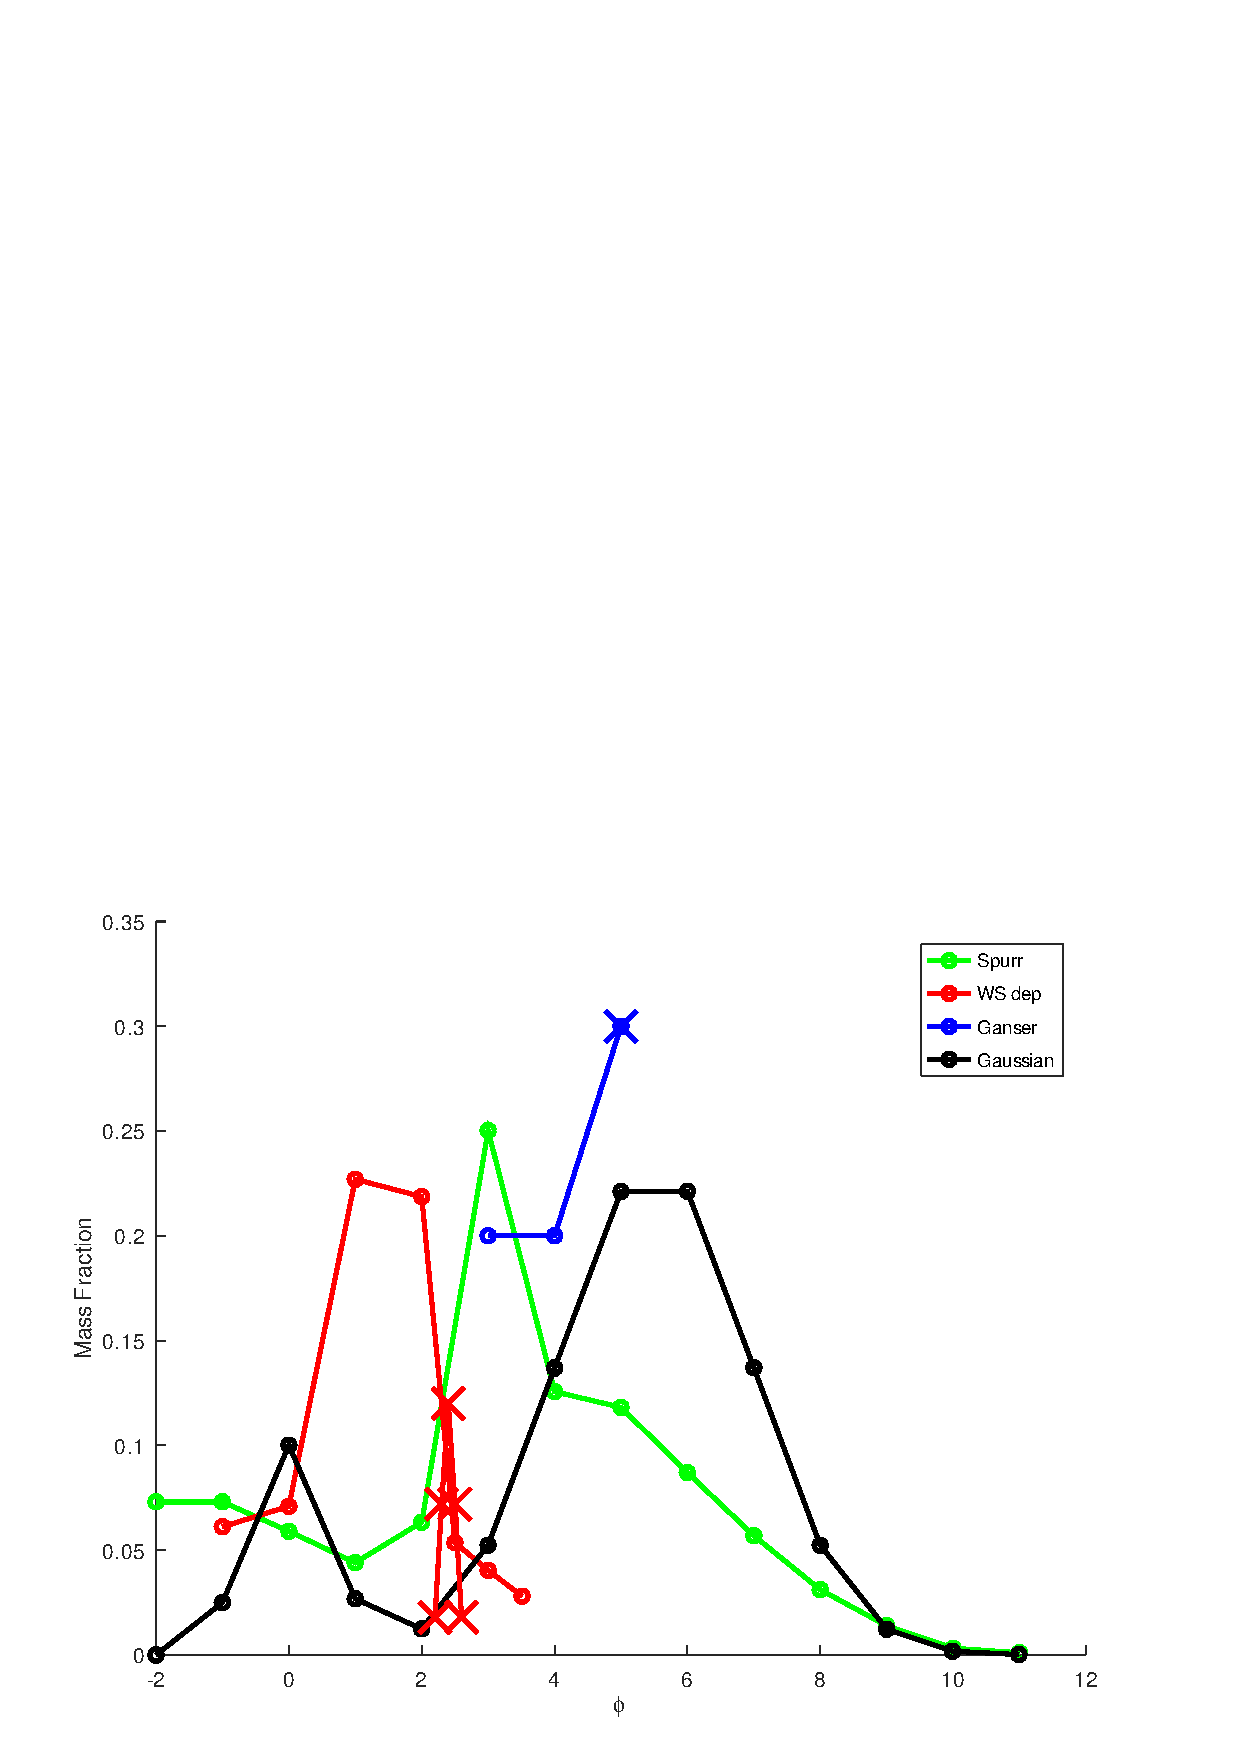
\includegraphics[angle=0,scale=0.7]{Figures/Scripts/InputGSD/FigInputGSD.pdf}
\parbox{15cm}{\caption{\label{FigInputGSD}
Example grain-size distributions.  The secondary populations (aggregates for the web
server deposit simulations and the flakes for the Ganser model) are shown with
crosses}}
\end{center}
\end{figure}

\paragraph{Block 8}: Locations of vertical profiles
In some cases it has been useful to plot vertical profiles through the ash cloud, as for
example, when ground-based LiDAR data were available over Europe during the 2010
eruption of Eyjafjallaj\"okull. In that case, the lines in Block 8 appeared as follows:

The first line contains an integer indicating the number of locations (nlocs) where
vertical profiles are to be recorded. If nlocs=0 (as in the example input file), no
lines follow in this block. Otherwise, nlocs lines follow, giving the locations for
each profile in the coordinate system appropriate for this model run (in this case,
degrees longitude and latitude, respectively). The blue comment lines give the names
of these locations.
Upon execution, Ash3d writes out text files with the names vprofile01.txt,
vprofile02.txt, vprofile03.txt, vprofile04.txt, containing vertical profiles at each
of these locations. Below is a truncated illustration of the output contained in
vprofile01.txt:

The header gives the x and y
coordinates of this location. The numbers in the first row of the table,
``0.250'', ``0.750'', ``1.250'', etc., are the elevations (km) of each cell center in the
model. Each row of data following contains the date and time (UTC, in yyyymmddhh.hh),
the number of hours after the beginning of the eruption, and the concentrations
(mg m-3) of tephra at each elevation. Ash3d writes out a line of output every 10 time
steps as long as the cloud is passing overhead.

\paragraph{Block 9}: Comment lines
Line 1 of this block gives the name of the output file containing the 3-D cloud
structure, if this output is specified in line 15 of Block 4.
Line 2 gives the title of the simulation. If the 3-D cloud structure is written
out to a NetCDF file (as specified in line 16 of Block 4), this title is included
in that file.
Line 3 gives an optional comment that may be written out to the same NetCDF file.

\paragraph{10+}: Optional modual blocks
After these required blocks have been read, Ash3d scans the input file to search
for the term ``\texttt{OPTMOD=}".  If this is found, then the corresponding optional
module input block is read.  This is primarily used in the development of
research branches of the code, but there are a few that are part of the main
code.

If a block with \texttt{OPTMOD=RESETPARAMS} is found, then a block of the input
file is read that allows the user to reset the default value of several global
variables.  For example, the following block would reset the default magma
density and deposit density.
\small
\begin{verbatim}
***********************
# Reset parameters
***********************
OPTMOD=RESETPARAMS
 MagmaDensity   = 3500.0
 DepositDensity = 1300.0
*******************************************************************************
\end{verbatim}
\normalsize

The full list of parameters than can be reset are given in Table \ref{tab:ResetParam}.
\small
\begin{table}[htbp]
\begin{center}
\begin{tabular}{| l | l | l | l |}
\hline
\texttt{name} & Default value & Units & Description \\
\hline
\texttt{MagmaDensity}      & 2500.0   & $\mathrm{kg/m^3}$  &  Density for DRE calculations\\
\texttt{DepositDensity}    & 1000.0   & $\mathrm{kg/m^3}$  &  Denisty of tephra deposit\\
\texttt{LAM\_GS\_THRESH}   & 250.0    & $\mathrm{m}$       &  mean free path for Cunningham slip\\
\texttt{AIRBORNE\_THRESH}  & 1.0e-3   & $\mathrm{kg}$      &  Airborne mass threshold for tracking\\
\texttt{GRAV}              & 9.81     & $\mathrm{m/s^2}$   &  Gravitational acceleration\\
\texttt{RAD\_EARTH}        & 6371.229 & $\mathrm{km}$      &  Radius of Earth\\
\texttt{CFL}               & 0.80     & unitless           &  Courant-Friedrick-Levy constant\\
\texttt{DT\_MIN}           & 1.0e-5   & $\mathrm{hour}$    &  Minimum allowed time-step\\
\texttt{DT\_MAX}           & 1.0      & $\mathrm{hour}$    &  Maximum allowed time-step\\
\texttt{ZPADDING}          & 1.3      & unitless           &  Scaling factor for height of z-grid\\
\texttt{DEPO\_THRESH}      & 1.0e-1   & $\mathrm{mm}$      &  Threshold value to output deposit\\
\texttt{DEPRATE\_THRESH}   & 1.0e-2   & $\mathrm{mm/hour}$ &  Threshold value to output deposit rate\\
\texttt{CLOUDCON\_THRESH}  & 2.0e-1   & $\mathrm{t/km^3}$  &  Threshold value to output cloud concentration\\
\texttt{CLOUDLOAD\_THRESH} & 2.0e-1   & $\mathrm{t/m^2}$   &  Threshold value to output cloud load\\
\texttt{THICKNESS\_THRESH} & 1.0e-2   & $\mathrm{mm}$      &  Threshold value to output deposit\\
\texttt{TOTCON\_THRESH}    & 1.0e-3   & $\mathrm{kg/km^3}$ &  Threshold value to output cloud load\\
\texttt{DBZ\_THRESH}       & -2.0e+1  & $\mathrm{dB}$      &  Threshold value to output radar reflectivity\\
\texttt{lambda}            & 0.2      & unitless           &  Suzuki constant for umbrella cloud\\
\texttt{N\_BV}             & 0.02     & $\mathrm{s^{-1}}$  &  Brunt-Va\"isala frequency for umbrella cloud\\
\texttt{k\_entrainment}    & 0.1      & unitless           &  Entrainment coefficient for umbrell cloud\\
\hline
\end{tabular}
\caption{\label{tab:ResetParam}Parameters than can be reset through \texttt{OPTMOD=RESETPARAMS}}
\end{center}
\end{table}
\normalsize

\paragraph{Environment variables}
Some variables can be set at run-time through the use of environment variables on a unix
system.  These are not needed, but can be used to change the default values if desired.
If the Ash3d executable was compiled to read the airport and volcano database files at
run-time, the path to these external files should be set when compiled.  The default is
\texttt{/opt/USGS/Ash3d}, but this is set in the \texttt{makefile} by the \texttt{INSTALLDIR}
variable.  If the files were subsequently moved, or if different versions were needed,
Ash3d tests for the environment variable \texttt{ASH3DHOME}.  Similarly, the CFL factor
is set by default to 0.8, but can be overwritten by the environment variable \texttt{ASH3DCFL}.
Note that this factor could be subsequently reset if the optional input block
\texttt{OPTMOD=RESETPARAMS} is used and \texttt{CFL} is set.

\paragraph{Executing Ash3d}
Run-time error checking
log file
stdout
stop conditions evaluation
finalization

%%%%%%%%%%%%%%%%%%%%%%%%%%%%%%%%%%%%%%%%%%%%%%%%%%%%%%%%%%%
\section{Post-processing}\label{ChapUsageSecPostProc}
kml files\\
processing ESRI ASCII files with GMT\\
processing NetCDF files with GMT\\
scripts from Ash3d\_web\\
conversion tool\\
tecplot

%AFWA GUI
